\chapter{Исследовательский раздел}
\label{cha:research}

\section{Примеры работы}
Рассмотрим примеры работы программы. На рисунках 4.1, 4.2, 4.3, 4.4 изображены случаи с двумя переставленными соседними буквами, пропущенной буквы, пустыми словами, и полностью разными словами соответственно.

\begin{figure}[H]
    \centering
    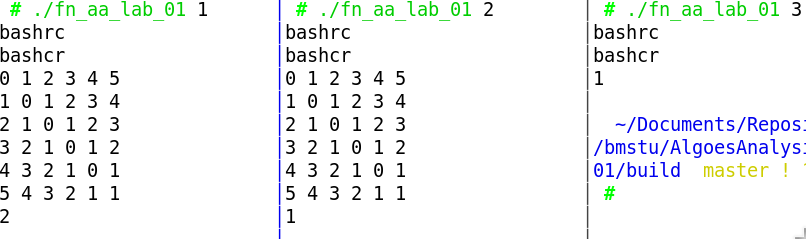
\includegraphics[scale=0.5]{./pics/t1.png}
    \caption{Транспозиция}
\end{figure}
\begin{figure}[H]
    \centering
    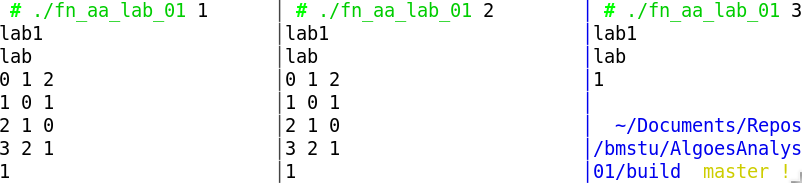
\includegraphics[scale=0.5]{./pics/t2.png}
    \caption{Пропуск одной буквы}
\end{figure}
\begin{figure}[H]
    \centering
    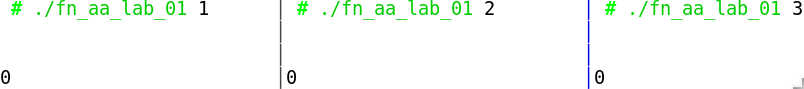
\includegraphics[scale=0.5]{./pics/t3.png}
    \caption{Пустые слова}
\end{figure}
\begin{figure}[H]
    \centering
    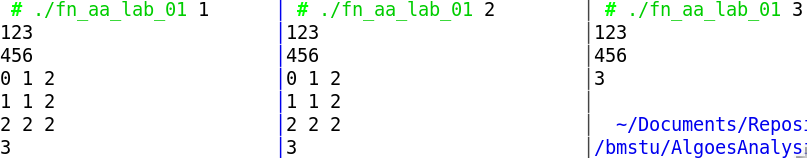
\includegraphics[scale=0.5]{./pics/t4.png}
    \caption{Совершенно разные слова}
\end{figure}

\section{Результаты тестирования}

\begin{table}[H]
    \caption{Результаты тестирования алгоритма Вагнера-Фишера}
	\begin{tabular}{|c|c|c|c|c|}
 	\hline
    \No{} & Строка 1 & Строка 2 & \makecell{Расстояние\\Левенштейна} & \makecell{Ожидаемое расстояние\\Левенштейна} \\
 	\hline
 	1 & some & any & 4 & 4\\
 	\hline
 	2 & & nothing & 7 & 7\\
 	\hline
 	3 & & & 0 & 0\\
 	\hline
 	4 & bashrc & bashcr & 2 & 2\\
 	\hline
 	5 & bus & BuS & 2 & 2\\
 	\hline
 	6 & electricity & city & 7 & 7\\
 	\hline
 	7 & powerful & powerless & 4 & 4\\
 	\hline
 	8 & grow & flow & 2 & 2\\
 	\hline
 	9 & rise & rice & 1 & 1\\
 	\hline
    10 & legal & illegal & 2 & 2\\
 	\hline
    11 & same & same & 0 & 0\\
    \hline
	\end{tabular}
\end{table}

\begin{table}[H]
    \caption{Результаты тестирования рекурсивного алгоритма Дамерау-Левенштейна}
	\begin{tabular}{|c|c|c|c|c|}
 	\hline
    \No{} & Строка 1 & Строка 2 & \makecell{Расстояние\\Дамерау-Левенштейна} & \makecell{Ожидаемое расстояние\\Дамерау-Левенштейна} \\
 	\hline
 	1 & some & any & 4 & 4\\
 	\hline
 	2 & & nothing & 7 & 7\\
 	\hline
 	3 & & & 0 & 0\\
 	\hline
 	4 & bashrc & bashcr & 1 & 1\\
 	\hline
 	5 & bus & BuS & 2 & 2\\
 	\hline
 	6 & electricity & city & 7 & 7\\
 	\hline
 	7 & powerful & powerless & 4 & 4\\
 	\hline
 	8 & grow & flow & 2 & 2\\
 	\hline
 	9 & rise & rice & 1 & 1\\
 	\hline
    10 & legal & illegal & 2 & 2\\
 	\hline
    11 & same & same & 0 & 0\\
    \hline
	\end{tabular}
\end{table}

\begin{table}[H]
    \caption{Результаты тестирования рекурсивного алгоритма Дамерау-Левенштейна}
	\begin{tabular}{|c|c|c|c|c|}
 	\hline
    \No{} & Строка 1 & Строка 2 & \makecell{Расстояние\\Дамерау-Левенштейна} & \makecell{Ожидаемое расстояние\\Дамерау-Левенштейна} \\
 	\hline
 	1 & some & any & 4 & 4\\
 	\hline
 	2 & & nothing & 7 & 7\\
 	\hline
 	3 & & & 0 & 0\\
 	\hline
 	4 & bashrc & bashcr & 1 & 1\\
 	\hline
 	5 & bus & BuS & 2 & 2\\
 	\hline
 	6 & electricity & city & 7 & 7\\
 	\hline
 	7 & powerful & powerless & 4 & 4\\
 	\hline
 	8 & grow & flow & 2 & 2\\
 	\hline
 	9 & rise & rice & 1 & 1\\
 	\hline
    10 & legal & illegal & 2 & 2\\
 	\hline
    11 & same & same & 0 & 0\\
    \hline
	\end{tabular}
\end{table}

